
\section{Translating CLASS to C}

Our work aims to improve the performance of CLASS programs by compiling them to native code, which can be executed directly on the target hardware.

As a first step, we focused on the translation of a subset of the CLASS language to GNU C.

\subsection{Overview}

Our CLASS compiler is built on top of the existing SAM and CLASS interpreter codebase. We reuse the existing lexer, parser and type checker, and extend it with a new code generation phase. Finally, the GNU C code outputted by the code generation phase is compiled using GCC to produce the final executable.

As CLASS has no notion of a call stack or function calls, the generated C programs have no functions other than the \texttt{main} function.
Instead, the computed \texttt{goto} construct % TODO reference this?
is used to jump between the two ends of each session. We call this action a \textit{session flip}.

To generate the code itself, we use the visitor pattern. The entry point of this phase is the \texttt{Generator} visitor, which traverses the typechecked CLASS AST, emitting C code for each node.
% TODO: clarify

\subsection{Execution Flow}



Different process definitions are generated within the \texttt{main} function. The program starts by initializing the environment for the entry process and immediately jumping to it.

Actions on a session can either be positive or negative. Positive actions are those that write to the session buffer, while negative actions are those that read from the session buffer.
Naturally, a positive action must always be executed before its negative counterpart, on the opposite end of the session.
To this end, the compiler generates code which performs a session flip whenever a negative action is encountered for the first time after the last positive action on the same session.

\subsubsection{Tasks}

When a parallel block is encountered, the compiler emits code for both the left-hand-side and right-hand-side processes, such that the left-hand-side process is executed first,
and the right-hand-side process execution is deferred into a new task which is pushed onto the task stack.

The task stack is implemented as a simple linked list, with each task containing:
\begin{itemize}
  \item A pointer to the next task to execute.
  \item A program address to jump to when executing the task.
  \item A pointer to the environment to switch to when executing the task.
\end{itemize}

When an empty process is encountered, which has no right-hand-side, the current task has finished, and thus the compiler emits code which pops the next task from the task stack and jumps to it.

To handle program termination, the task stack is initialized with a single task which jumps to the end of the program.

\subsubsection{Process Definition Calls}

When a process definition call is encountered, the compiler first checks the polarity of the process definition arguments.
For each negative argument, for which we previously wrote to, the compiler emits code to flip the session.
Then, the compiler emits code to initializes a new environment for the process definition, and jumps to it.
This environment is initialization is done by simply assigning the session names of the new environment to the names of the arguments in the current environment.

\subsection{Session Queues}

One of the key design decisions in the translation process is the representation of sessions. On our implementation, for each session we allocate a buffer with a size determined at compile time. This buffer acts as queue where the writer side of the session appends data to, so that the reader side can read it later.



\subsection{Data Structures}

The programs generated by the compiler use a number of data structures to describe their state.

\vspace{1em}

A environment contains:
\begin{itemize}
  \item A mapping from session names (indices) to pointers to linear session records.
  \item A mapping from type variable names (indices) to their polarity.
  \item A pointer to the first exponential session record, if one exists.
\end{itemize}

\vspace{1em}

An exponential session record contains:
\begin{itemize}
  \item A pointer to the parent exponential session record.
  \item A program address to initialize linear instances of the 
\end{itemize}

\vspace{1em}

A linear session record contains:
\begin{itemize}
  \item A program address to jump to on the next session flip.
  \item A pointer to the environment to switch to on the next session flip.
  \item The name (index) of the session in the environment above.
  \item The base address of the session's buffer.
\end{itemize}

% \begin{figure}
%   \centering
%   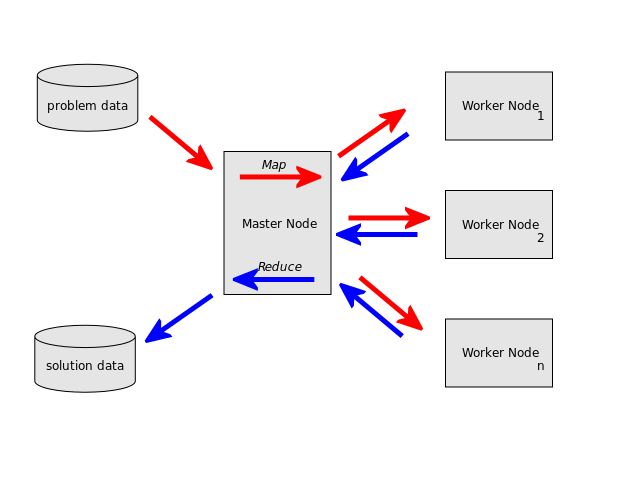
\includegraphics[width=0.6\textwidth]{Images/overview.png}
%   \caption{Solution Overview}
%   \label{fig:Scheme}
% \end{figure}
